\chapter{WORK SCHEDULE}
\begin{figure}[ht]
\centering
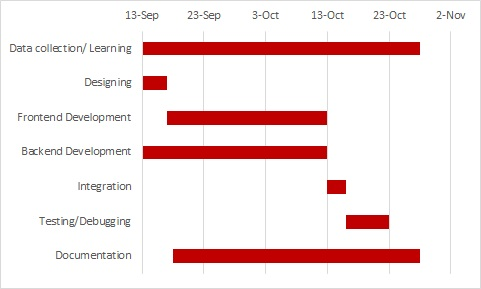
\includegraphics[width=\linewidth]{Graphics/time.JPG}
\caption{Time schedule }
\end{figure}

\begin{enumerate}[label=(\alph*)]
	\item Data Collection/Learning refers to the data being added to the database in order to make the application and learning how to apply them. Since this can go concurrently with other works being done and takes less time than others, it is taking full project time.
	\item Designing is the time for making UI/UX for frontend developement. It has been given 4 days since we are using Agile model, this could be improved on later iteration. It starts on the first day of the project.
	\item Frontend Development is the part to code the interface costumers see and act on. Since it is connected with designing part it's given 26 days giving interface development 1 month to complete. 
	\item Backend Development is the part where all of the data are stored and is needed to be kept secure. Hence, all of the 1 month is given to this task and it starts on the first day of the project. Team is divided into frontend and backend so that things could be done concurrently.
	\item Integration is the part of combining frontend and backend of the program. Several Errors might occur hence, 3 days are given for this.
	\item Testing/Debugging is the part where anyone except the development group is given the application to try and if bug is found it is patched out.
	\item Documentation is the part of writing down everything that has been done in the project hence making it easier for debugging and changing on future iterations.
\end{enumerate}
 